\documentclass[a4paper]{article}
\usepackage{fullpage}
\usepackage[T1]{fontenc}
\usepackage[utf8]{inputenc}

\usepackage{lmodern}

% For TikZ diagrams:
\usepackage{pgfplots}
\pgfplotsset{compat=1.11}

\title{A Probabilistic Micropayment Scheme for Golem}
\author{Golem Team (\texttt{golem@imapp.pl})}

\begin{document}
\maketitle

\begin{abstract}
  We consider a setting where a transaction is made by a single payer
  to a possibly large group of recipients, each receiving only a small
  sum in the order of \$$0.01$. For such small sums transaction fees are
  relatively large even if we consider cryptocurrencies instead of
  bank-based transactions.

  Both payers and recipients are expected to repeatedly take part in
  many transactions, but subsequent transactions of a single payer may
  have different, possibly disjoint, groups of recipients. Also, we
  assume that transactions result from activities carried out in a
  decentralized peer-to-peer network, so we would like to avoid
  solutions relying on any trusted third party. We cannot therefore use
  existing solutions that require a central server or assume that a
  payer makes a series of micropayments to a single recipient (Bitcoin
  micropayment channels).

  Instead, we propose a probabilistic payment scheme in which only one
  recipient randomly chosen from a group of candidates is rewarded in
  a single transaction. Our solution is based on Ethereum and is thus
  decentralized and avoids relying on a trusted third party. In
  particular, we describe an Ethereum smart contract implementing a
  lottery used to reward recipients. In the proposed payment scheme,
  the estimated cost of ...\marginpar{dokończyć zdanie}
\end{abstract}

\begin{figure}
  % Merkle tree example for the micropayments Golem paper
% Requires \usepackage{pgfplots} 

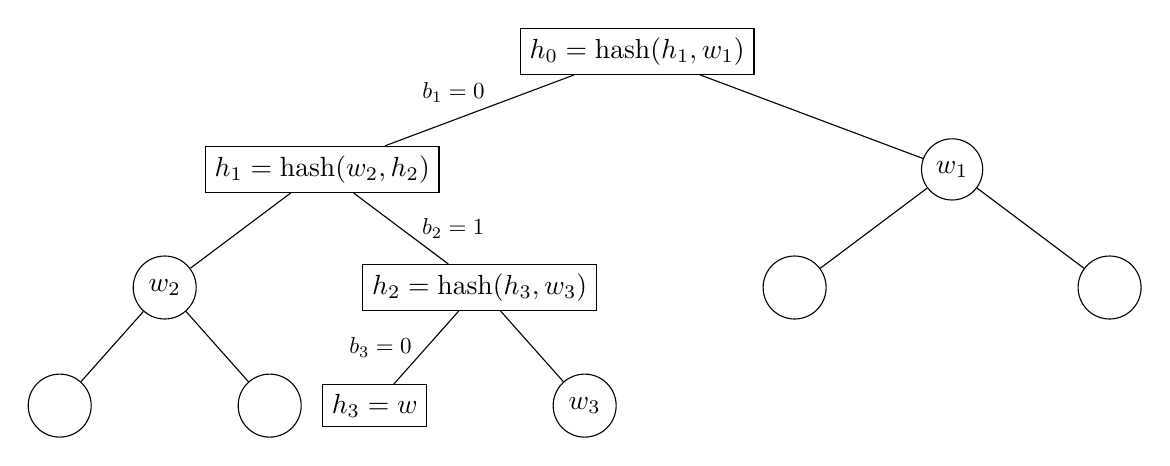
\begin{tikzpicture}[level/.style={sibling distance=8cm/#1}]
\newcommand{\hash}[1]{\mathrm{hash}({#1})}
\node [rectangle, draw] (c)  {$h_0 = \hash{h_1, w_1}$}
	child { node [rectangle, draw] (l)  {$h_1 = \hash{w_2, h_2}$}  
		child { node [circle, draw, minimum size=0.8cm] (ll) {$w_2$} 
			child { node [circle, draw, minimum size=0.8cm] (lll) {}}
			child { node [circle, draw, minimum size=0.8cm] (llr) {}}
		}
		child { node [rectangle, draw] (B)  {$h_2 = \hash{h_3, w_3}$} 
			child { node [rectangle, draw] (lrl) {$h_3 = w$} 
				edge from parent node[scale=0.83, left=0.1cm] {$b_3= 0$}	
			}
			child { node [circle, draw, minimum size=0.8cm](lrr) {$w_3$}}
			edge from parent node[scale=0.83, right=0.2cm] {$b_2= 1$}	
		}
		edge from parent node[scale=0.83, left=0.4cm, above=0.0cm] {$b_1 = 0$}	
	}
	child { node [circle, draw] (r) {$w_1$}
		child { node [circle, draw, minimum size=0.8cm] (rl) {$$}
		 }
		child { node [circle, draw, minimum size=0.8cm] (rr)  {$$}
		} 
	}
;
\end{tikzpicture}

  \caption{An example Merkle tree.}
  \label{fig:merkle}
\end{figure}

Figure~\ref{fig:merkle} shows an example Mekle tree with a distinguished node $n = 010$. Its label $w$, together with labels $w_3$, $w_2$ and $w_1$ are used to compute hashes $h_3, \ldots, h_0$.

\end{document}
